\section{Filter-Approximationen im Detail}

\subsection{Approximation mittels kritisch-gedämpfter Filter}{299}

Tiefpassfilter $n.$ Ordnung mit kritischer Dämpfung haben jeweilen einen $\bm{n}$\textbf{-fachen Pol} auf der \textbf{negativen}
$\sigma$-Achse.

\begin{itemize}
    \item Impuls- und Sprungantwort können nicht oszillieren
    \item Geringe Flankensteilheit im Übergangsbereich
\end{itemize}
\vspace{0.2cm}

Die Übertragungsfunktion $H(s)$ ergibt sich als:

\begin{minipage}[c]{0.48\columnwidth}
    $$ \boxed{ H(s) = \frac{1}{\Big( 1 + \frac{s}{\omega_c} \Big)^n} } $$
\end{minipage}
\hfill
\begin{minipage}[c]{0.48\columnwidth}
    \begin{tabular}{ll}
        $n$         & Ordnung des Filters \\
        $\omega_c$  & $3 \, \deci \bel$-Punkt jedes der $\bm{n}$ \textbf{Teilfilter}
    \end{tabular}
\end{minipage}

\vspace{0.2cm}
Will man bei der Kreisfrequenz $\omega_D$ eine Dämpfung von $\alpha \, \deci \bel$ haben, so muss $\omega_c$ (der $n$ identischen
Teilfilter) gewählt werden als
$$ \boxed{ \omega_c = \frac{\omega_D}{\sqrt{10^{\frac{\alpha}{10 \cdot n}} -1}} } $$ 


\subsubsection{Eigenschaften kritisch-gedämpfte Filter}

\begin{itemize}
    \item Alle Pole am \textbf{gleichen Ort} auf negativer $\sigma$-Achse \textrightarrow\ Allpolfilter
    \item Für $\Omega = 0$ ist für sämtliche $n$: $|H(0)| = H_{\max} = 1$
    \item Für $\Omega = 1$ ist für sämtliche $n$: $|H(\jimg)| = \frac{H_{\max}}{\sqrt{2}} = \frac{1}{\sqrt{2}}$
        \textrightarrow\ $3 \, \deci \bel$ Dämpfung
    \item Für $\Omega \gg 1$ wird $|H(\jimg \Omega)| \approx \frac{1}{\Omega^n}$ \textrightarrow\ $\bm{- n \cdot 20 \, \deci \bel /}$ \textbf{Dekade}
    \item Amplitudengang bei $\Omega = 0$ maximal flach, da alle Ableitungen $=0$ sind
    \item Amplitudengang ist streng-monoton fallend \textrightarrow\ keine Welligkeit
    \item Pole verschieben sich bei höherer Ordnung näher in Richtung imaginäre Achse
    \item Gruppenlaufzeit konstant bis $\omega_D$
\end{itemize}


\begin{minipage}[c]{0.4\columnwidth}
    \begin{center}
        \textbf{\myul{Amplitudengänge}}
    \end{center}
    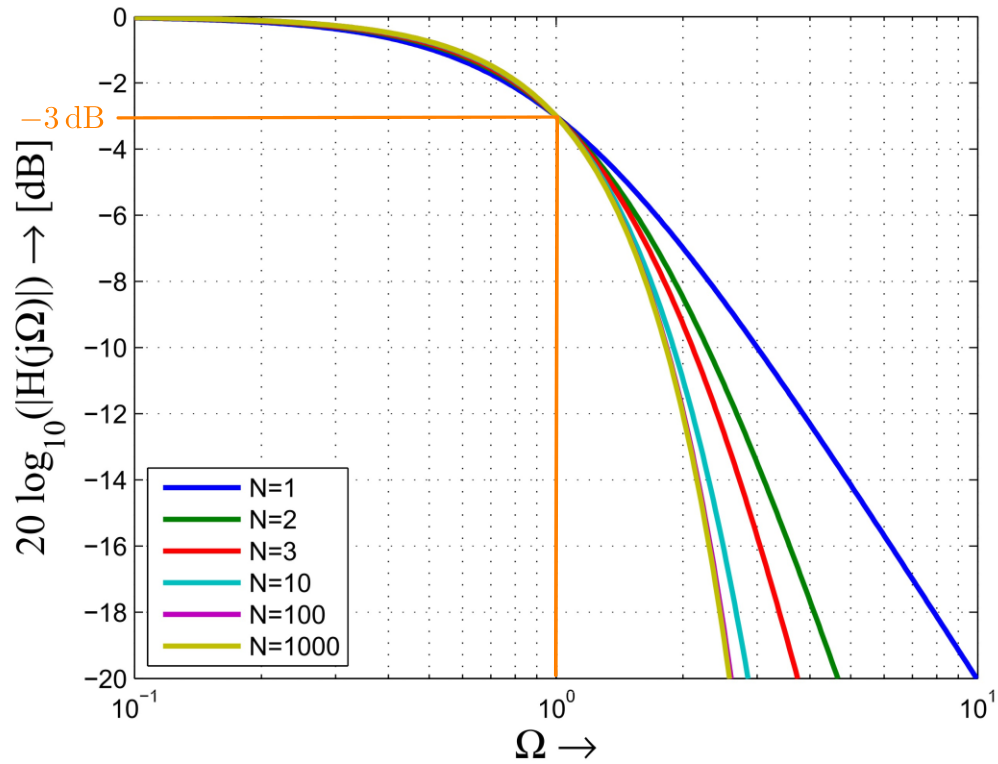
\includegraphics[width=\columnwidth]{images/filter_kritisch_gedaempft_normierter_amplitudengang.png}
\end{minipage}
\hfill
\begin{minipage}[c]{0.4\columnwidth}
    \begin{center}
        \textbf{\myul{Pol-Lagen}}
    \end{center}
    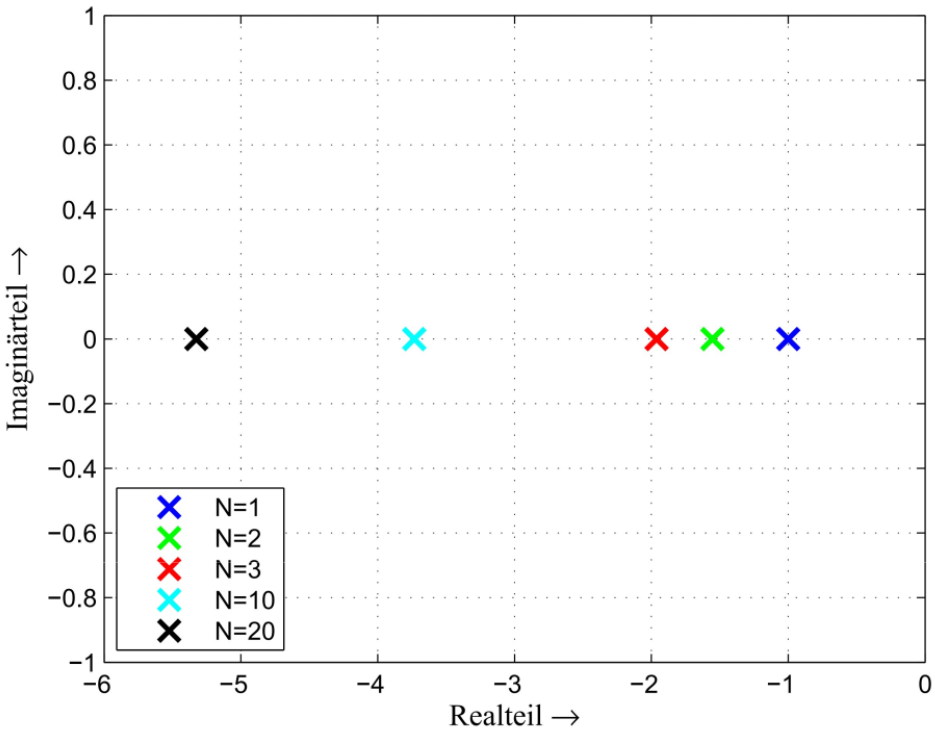
\includegraphics[width=\columnwidth]{images/filter_kritisch_gedaempft_pollagen.png}
\end{minipage}


\subsection{Approximation nach Butterworth}{303}

\begin{minipage}[c]{0.45\columnwidth}
    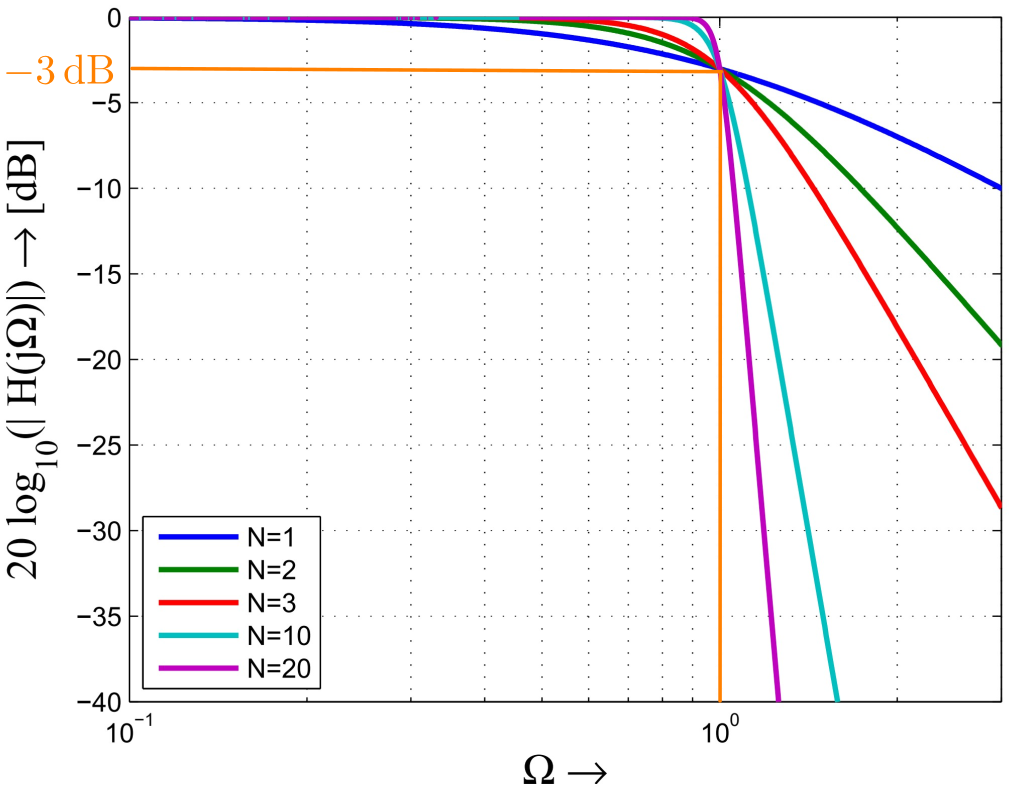
\includegraphics[width=\columnwidth]{images/filter_butterworth_amplitudengang.png}
\end{minipage}
\hfill
\begin{minipage}[c]{0.48\columnwidth}
    Die charakteristische Funktion wird bei der Butterworth-Approximation als\\
    $K(\Omega^2) = (\Omega^2)^n = \Omega^{2n}$ gewählt.

    Der Amplitudengang $|H(\jimg \Omega)|$ folgt somit der Gleichung

    $$\boxed{ |H(\jimg \Omega)| = \frac{1}{\sqrt{ 1 +\Omega^{2n}}} } $$
\end{minipage}


\subsubsection{Eigenschaften der Butterworth-Approximation}{303}

\begin{outline}
    \1 \textbf{Durchlassbereich}
        \2 Für $\Omega = 0$ ist für sämtliche $n$: $|H(0)| = H_{\max} = 1$
        \2 Für $\Omega = 1$ ist für sämtliche $n$: $|H(\jimg)| = \frac{H_{\max}}{\sqrt{2}} = \frac{1}{\sqrt{2}}$
            \textrightarrow\ $3 \, \deci \bel$ Dämpfung
        \2 Amplitudengang bei $\Omega = 0$ maximal flach, da alle Ableitungen $=0$ sind

    \1 \textbf{Sperrbereich}
        \2 Für $\Omega \gg 1$ wird $|H(\jimg \Omega)| \approx \frac{1}{\Omega^n}$ 
            \textrightarrow\ $\bm{- n \cdot 20 \, \deci \bel /}$ \textbf{Dekade}
    \1 \textbf{Allgemein}
        \2 Amplitudengang ist streng-monoton fallend \textrightarrow\ keine Welligkeit
\end{outline}


\subsubsection{Bestimmung von $H(s)$ aus $|H(\jimg \Omega)|$}{304}
\label{Bestimmung UTF aus Amplitudengang}

Aus dem Ansatz 
$$ | H(\jimg \Omega) |^2 = \frac{1}{1 + K(\Omega^2)} \Big|_{\Omega^2 = -S^2} = \frac{1}{1 + (-S^2)^n} = \cbl{H(S)} \cdot H(-S)
    = \cbl{\frac{1}{D(S)}} \cdot \frac{1}{D(-S)} $$
kann der folgende Teil isoliert betrachtet werden ($D(S)$ ist ein Hurwitz-Polynom):
$$ \boxed{ D(S) \cdot D(-S) = 1 + (-S^2)^n } $$

Mit dem Ansatz 
$$ \boxed{ D(S) = \prod\limits_{j=1}^{t} (S^2 + a_j \cdot S + b_j) \prod\limits_{j=2t+1}^{n} (S - c_j) } $$
wird das Produkt $D(S) \cdot D(-S)$ bestimmt. Anschliessend wird ein Koeffizientenvergleich durchgeführt.

\subsubsection{Bestimmung der Pol-Lage}{307}

Der Zusammenhang aus Abschnitt~\ref{Bestimmung UTF aus Amplitudengang} kann für die Bestimmung der Pole auf Null gesetzt werden:
$$ \boxed{ D(S) \cdot D(-S) = 1 + (-S^2)^n \overset{!}{=} 0 } $$
Durch Auflösen der Gleichung nach $S$ kommen die Pole auf dem \textbf{Einheitskreis} zu liegen.

\begin{itemize}
    \item Abstand zwischen den Polen: $\frac{\pi}{n}$
    \item Ordnung $n$ gerade: keine reellen Pole
    \item Ordnung $n$ ungerade: zwei reelle Pole bei $\pm 1$
    \item \textbf{Für Nennerpolynom $\bm{D(S) = \frac{1}{H(S)}}$ müssen nur Pole in der linken Halbebene berücksichtigt werden!}
\end{itemize}

\begin{center}
    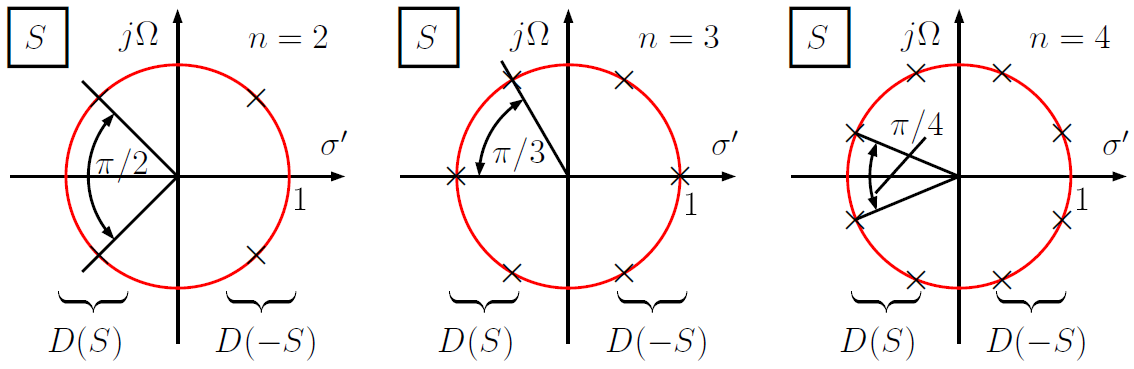
\includegraphics[width=0.8\columnwidth]{images/filter_pollage_butterworth.png}
\end{center}


\example{Butterworth 2. Ordnung -- $H(s)$ und Pol-Lage bestimmen}

$$ \text{Ansatz:} \quad H(S) \cdot H(-S) = \frac{1}{D(S)} \cdot \frac{1}{D(S)} = \frac{1}{ 1 + (-S^2)^n} $$

Für die Ordnung $n = 2$ ergibt sich das Nennerpolynom zu:
$$ D(S) \cdot D(-S) = 1 + S^4 \quad \Leftrightarrow \quad S^4 = -1 \quad \Leftrightarrow \quad
    e^{\jimg \bigl( \frac{\pi}{4} + k \frac{\pi}{2} \bigr)}$$

\begin{minipage}[c]{0.3\columnwidth}
    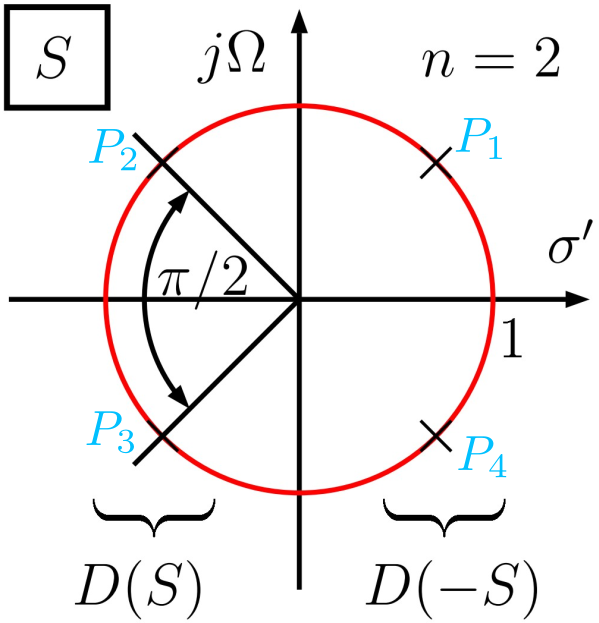
\includegraphics[width=\columnwidth]{images/filter_butterworth_pollagen_ordnung_2.png}
\end{minipage}
\hfill
\begin{minipage}[c]{0.58\columnwidth}
    Aufgelöst nach $S$ liegen die Nullstellen auf dem Einheitskreis mit Abstand $\frac{\pi}{4}$ verteilt.
    \vspace{0.2cm}

    \renewcommand{\arraystretch}{1.3}
    \begin{tabular}{c c}
        \textbf{Rechte Halbebene}                             & \textbf{Linke Halbebene} \\
        $P_1 = \frac{1}{\sqrt{2}} + \jimg \frac{1}{\sqrt{2}}$ & $P_2 = - \frac{1}{\sqrt{2}} + \jimg \frac{1}{\sqrt{2}}$ \\
        $P_4 = \frac{1}{\sqrt{2}} - \jimg \frac{1}{\sqrt{2}}$ & $P_3 = - \frac{1}{\sqrt{2}} - \jimg \frac{1}{\sqrt{2}}$ \\
    \end{tabular}
    \renewcommand{\arraystretch}{1}

    \vspace{0.2cm}
    \textrightarrow\ Für die Übertragungsfunktion $H(s)$ sind nur die Nullstellen in der \textbf{linken Halbebene} relevant!
\end{minipage}

\vspace{0.2cm}
Die Übertragungsfunktion $H(S)$ ergibt sich aus
$$ H(S) = \frac{1}{D(S)} = \frac{1}{(S - P_2) \cdot (S - P_3)} = \frac{1}{S^2 + \sqrt{2} S + 1} $$


Alternativ kann die Übertragungsfunktion $H(S)$ auch mittels folgendem Ansatz für $D(S)$ und anschliessendem Koeffizientenvergleich
von $D(S) \cdot D(-S)$ bestimmt werden.

$$ \text{Ansatz:} \quad  D(S) =  S^2 + a_1 S + b_1 $$
$$ \text{Koeffizientenvergleich:} \quad D(S) \cdot D(-S) = S^4 + (2 b_1 - a_1^2) \, S + b_1^2 \overset{!}{=} S^4 + 1 $$
\textrightarrow\ $a_1 = \sqrt{2}$ und $b_1 = 1$ \quad \textrightarrow\ $S^2 + \sqrt{2} S + 1$ 
\quad \textrightarrow\ $H(s) = \frac{1}{D(s)} = \frac{1}{S^2 + \sqrt{2} S + 1}$


\subsubsection{Bestimmung der Filterordnung}{308}

Aus dem Toleranzschema lassen sich für die 'Ecken' die folgenden beiden Bedingungen aufstellen:

\begin{minipage}[c]{0.48\columnwidth}
    $$ A(\Omega_D) = 10 \cdot \log_{10}(1 + \Omega_D^{2n}) = A_{pass} $$
\end{minipage}
\hfill
\begin{minipage}[c]{0.48\columnwidth}
    $$ A(\Omega_S) = 10 \cdot \log_{10}(1 + \Omega_S^{2n}) = A_{stop} $$
\end{minipage}

\vspace{0.2cm}
\begin{minipage}[c]{0.48\columnwidth}
    Mittels Umformungen und aufgelöst nach $n$ ergibt sich die Filter-Ordnung als 

    \medskip
    $\left\lceil . \right\rceil $ bedeutet '\textbf{aufrunden} auf ganze Zahl' (ceil()-Funktion)
\end{minipage}
\hfill
\begin{minipage}[c]{0.48\columnwidth}
    $$ \boxed{ n =  \left\lceil \frac{\log_{10} \Bigl( \frac{10^{A_{stop }/ 10} - 1}{10^{A_{pass}/ 10} - 1}  \Bigr) }
        {2 \cdot \log_{10}\Bigl( \frac{\Omega_S}{\Omega_D} \Bigr)}  \right\rceil } $$
\end{minipage}

\textrightarrow\ Alternativ kann die Ordnung $n$ auch mit dem \textbf{Nomogramm} bestimmt werden.

% --------------------------------------------------------------------------------------------------
\subsection{Approximation nach Tschebyscheff-\uproman{1}}{310}

\begin{minipage}[c]{0.45\columnwidth}
    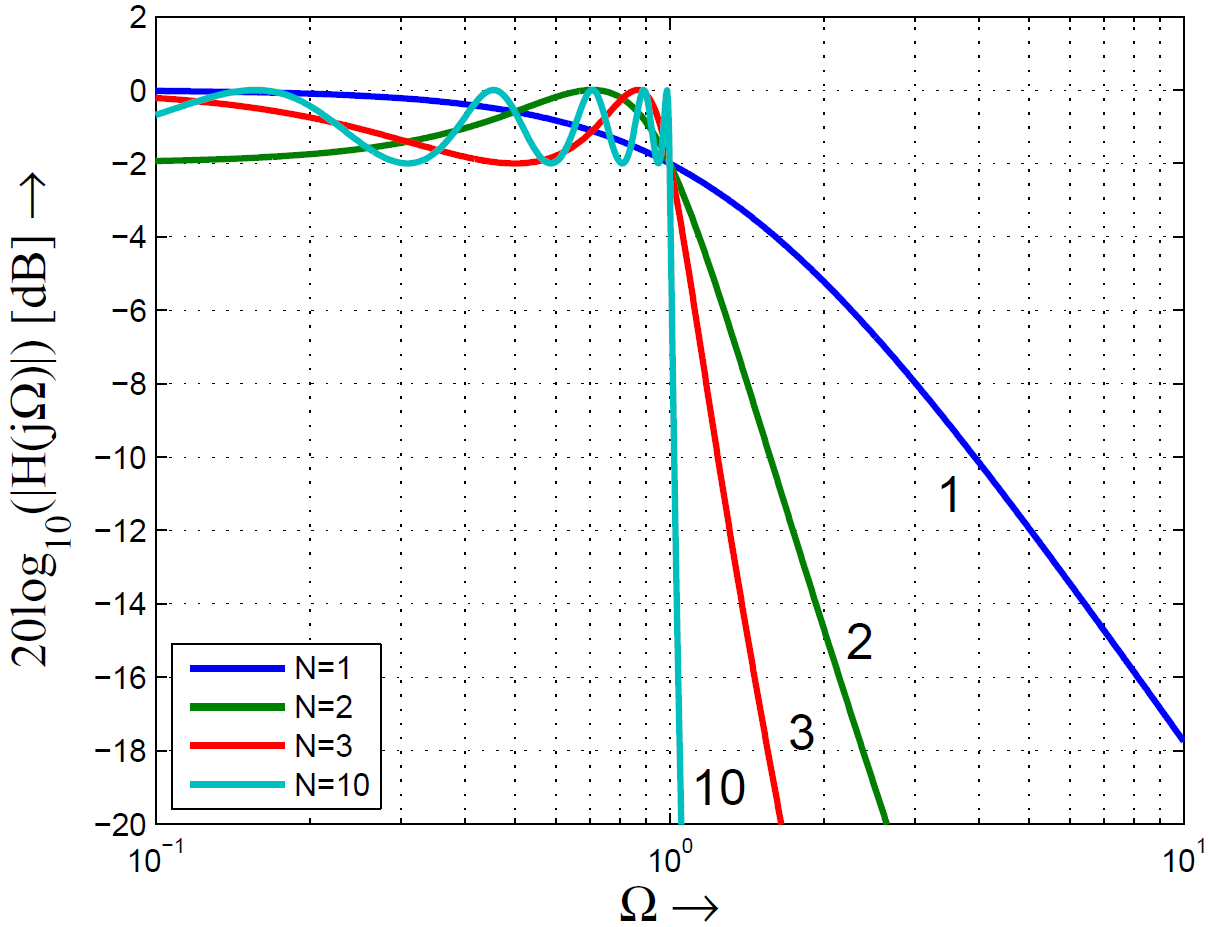
\includegraphics[width=\columnwidth]{images/filter_tschebyscheff_amplitudengang.png}
\end{minipage}
\hfill
\begin{minipage}[c]{0.48\columnwidth}
    Die charakteristische Funktion wird bei der Tschebyscheff-\uproman{1} als\\
    $K(\Omega^2) = e^2 \cdot C_n^2(\Omega)$ gewählt.

    Der Amplitudengang $|H(\jimg \Omega)|$ folgt somit der Gleichung

    $$\boxed{ |H(\jimg \Omega)| = \frac{1}{\sqrt{1 + e^2 \cdot C_n^2(\Omega)} } } $$

    \begin{tabular}{ll@{}}
        $e$             & \textbf{Rippelfaktor} (Konstante) \\
        $C_n(\Omega)$   & Tschebyscheff-Polynom erster\\
                        & Art der Ornung $n$
    \end{tabular}
\end{minipage}

Das Tschebyscheff-Polynom $C_n(\Omega)$ ist im Durchlassbereich und im Sperrbereich \textbf{unterschiedlich definiert!}

\vspace{0.2cm}

\begin{minipage}[c]{0.48\columnwidth}
    \begin{center}
        \myul{Duchlassbereich $(|\Omega| \leq 1)$}
        $$ \boxed{ C_n(\Omega) = \cos(n \cdot \arccos(\Omega)) } $$
    \end{center}
    
\end{minipage}
\hfill
\begin{minipage}[c]{0.48\columnwidth}
    \begin{center}
        \myul{Sperrbereich $(|\Omega| \geq 1)$}
        $$ \boxed{ C_n(\Omega) = \cosh(n \cdot \mathrm{arccosh}(\Omega)) } $$
    \end{center}
\end{minipage}

\vspace{0.2cm}
Für die Ordnung $n \geq 2$ lässt sich das Tschebyscheff-Polynom $C_n(\Omega)$ mittels Rekursionsformel berechnen
$$ \boxed{ C_n(\Omega) = 2 \, \Omega \, C_{n-1}(\Omega) - C_{n-2}(\Omega) }  \qquad C_0(\Omega) = 1 \qquad C_1(\Omega) = \Omega $$

Zwischen dem Rippelfaktor $e$ und der maximalen Dämpfung $A_{\max}$ gilt der Zusammenhang:
$$ \boxed{ A_{\max} = 10 \cdot \log_{10}(1 + e^2) \quad \Leftrightarrow \quad e = \sqrt{10^{\frac{A_{\max}}{10}} -1} } $$


\subsubsection{Eigenschaften der Tschebyscheff-\uproman{1}-Approximation}{311}

Im \textbf{Durchlassbereich} schwankt das Tschebyscheff-Polynom in den Grenzen $\pm 1$. Im \textbf{Sperrbereich} nimmt
$C_n$ monoton mit $\Omega$ zu.

\begin{center}
    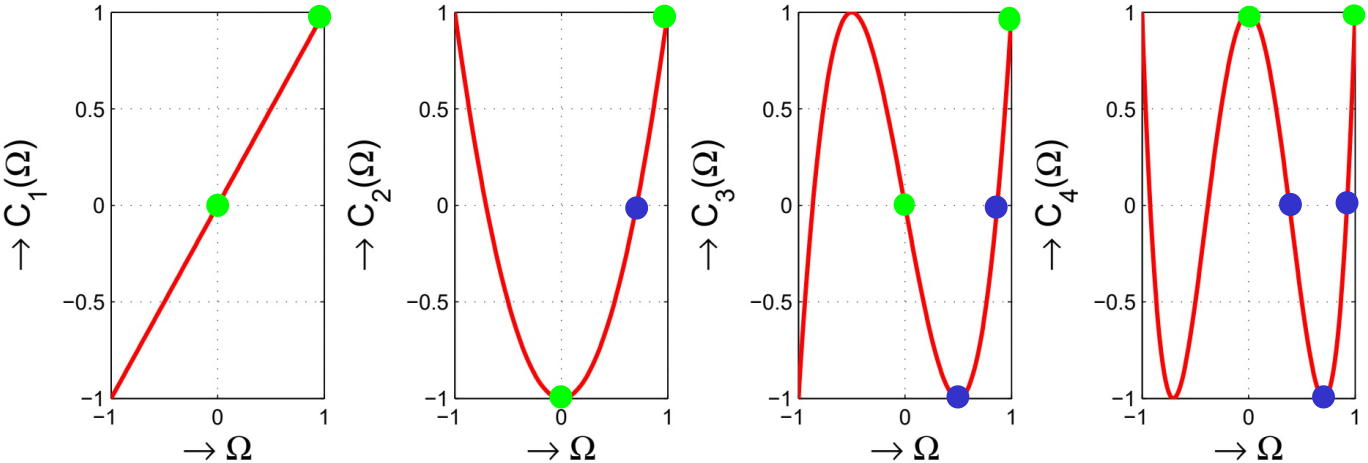
\includegraphics[width=0.8\columnwidth]{images/filter_tschebyscheff_ordnung_ablesen.png}
\end{center}


\begin{outline}
    \1 \textbf{Durchlassbereich}
        \2 Für $\Omega = 0$ ist für \textbf{un}gerade $n$: $|H(0)| = H_{\max} = 1$
        \2 Für $\Omega = 0$ ist für gerade $n$: $|H(0)| = \frac{1}{\sqrt{1 + e^2}}$
        \2 Für $\Omega = 1$ ist für sämtliche $n$: $|H(\jimg)| = \frac{1}{\sqrt{1 + e^2}}$ 
            \textrightarrow\ \textbf{nicht} $3 \, \deci \bel$ Dämpfung
        \2 Aus der Anzahl \textbf{\cbl{Wendepunkte} und \cgn{Endpunkte}} des Amplitudengangs im \textbf{Durchlassbereich} 
            $(0 \leq \Omega \leq 1)$ lässt sich die \textbf{Ordnung $\bm{n}$} bestimmen. \\
            \textbf{Ordnung = (Summe aller \cbl{Wendepunkte}) plus beide \cgn{Endpunkte} minus 1}
    \1 \textbf{Sperrbereich}
        \2 Für $\Omega \gg 1$ wird $|H(\jimg \Omega)| \approx \frac{1}{e \cdot C_n(\Omega)}$ 
            \textrightarrow\ $\bm{- n \cdot 20 \, \deci \bel /}$ \textbf{Dekade} bzw.\\
            $\bm{- n \cdot 6.02 \, \deci \bel /}$ \textbf{Oktave}
        \2 Fixe Ordnung $n$: Je grösser der Rippelfaktor $e$, desto steiler der Abfall in den Sperrbereich
        \2 Fixer Rippelfaktor $e$: Je grösser die Ordnung $n$, desto steiler der Abfall in den Sperrbereich
\end{outline}


\begin{minipage}[t]{0.48\columnwidth}
    \subsubsection{Pol-Lagen}{313}

    \begin{itemize}
        \item Die Pole liegen auf einer \textbf{Ellipse}
        \item Allpolfilter
        \item Je näher die Pole an der $\jimg \omega$-Achse liegen, desto mehr Rippel gibt es im Phasengang %CHECK: Phasengang oder Amplitudengang?
    \end{itemize}
\end{minipage}
\hfill
\begin{minipage}[t]{0.48\columnwidth}
    \subsubsection{Filterordnung}{316}

    $$ \boxed{ n =  \left\lceil \frac{\operatorname{arcosh} \Bigl( \sqrt{ \frac{10^{A_{stop}/ 10} - 1}{10^{A_{pass}/ 10} - 1} } \Bigr) }
        {\operatorname{arcosh} \Bigl( \frac{\Omega_S}{\Omega_D} \Bigr)}  \right\rceil } $$
    \textrightarrow\ \textbf{Nomogramme!}
\end{minipage}


\subsection{Approximation nach Tschebyscheff-\uproman{2}}{319}

\begin{minipage}[c]{0.45\columnwidth}
    \textbf{Inverses Tschebyscheff-Filter}

    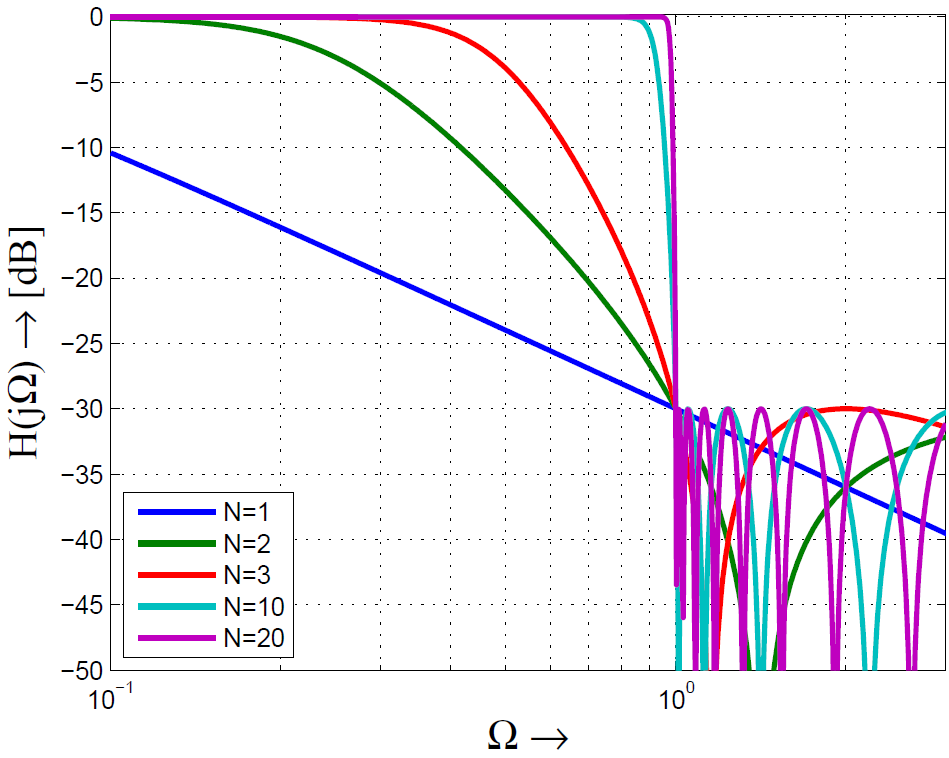
\includegraphics[width=\columnwidth]{images/filter_tschebyscheff_invers_amplitudengang.png}
\end{minipage}
\hfill
\begin{minipage}[c]{0.48\columnwidth}
    Die charakteristische Funktion wird bei der Tschebyscheff-\uproman{2}-Approximation als\\
    $K(\Omega^2) = e^2 \cdot C_n^2(\Omega)$ gewählt.

    Der Amplitudengang $|H(\jimg \Omega)|$ folgt somit der Gleichung

    $$ \boxed{ |H(\jimg \Omega)| = \frac{1}{\sqrt{1 + \frac{1}{e^2 C_n^2  \big(\frac{1}{\Omega} \big) }}} } $$

    \begin{tabular}{ll@{}}
        $e$             & \textbf{Rippelfaktor} (Konstante) \\
        $C_n(\Omega)$   & Tschebyscheff-Polynom erster\\
                        & Art der Ornung $n$
    \end{tabular}
\end{minipage}


\subsubsection{Lage der Pole und Nullstellen}{321}

\begin{minipage}[c]{0.4\columnwidth}
    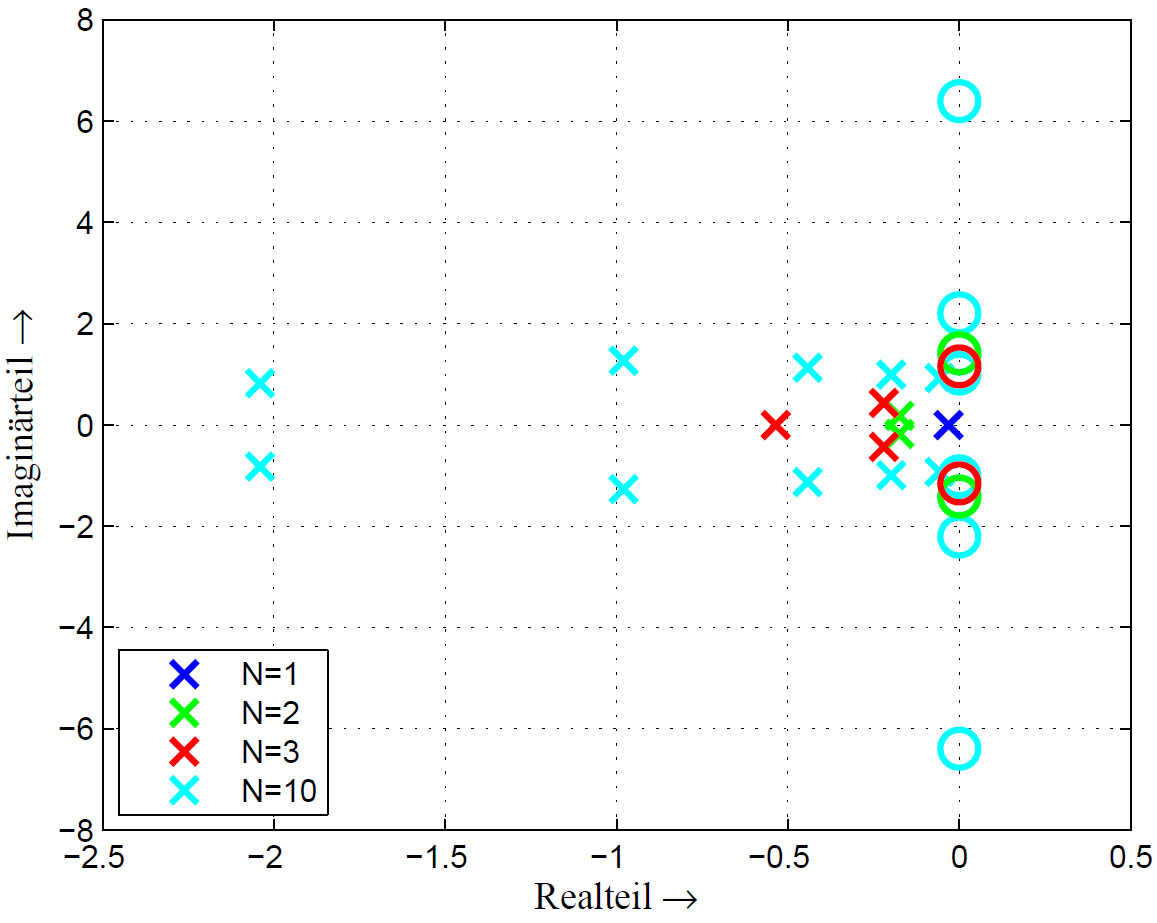
\includegraphics[width=\columnwidth]{images/filter_tschebyscheff_invers_pollage.png}
\end{minipage}
\hfill
\begin{minipage}[c]{0.58\columnwidth}
    \begin{outline}
        \1 \textbf{Kein} Allpolfilter
            \2 Gerade Ordnung $n$: $n$ Pole und $n$ Nullstellen
            \2 \textbf{Un}gerade Ordnung $n$: $n$ Pole und $n-1$ Nullstellen
    \end{outline}
\end{minipage}


\subsubsection{Filterordnung}{319}

\begin{minipage}[c]{0.4\columnwidth}
    $$ \boxed{ n =  \left\lceil \frac{\arccos \Bigl( \sqrt{ \frac{10^{A_{stop }/ 10} - 1}{10^{A_{pass }/ 10} - 1} } \Bigr) }
    {\arccos \Bigl( \frac{\Omega_S}{\Omega_D} \Bigr)}  \right\rceil } $$
\end{minipage}
\hfill
\begin{minipage}[c]{0.58\columnwidth}
    Die Filterordnung berechnet sich identisch wie bei der Tschebyscheff-\uproman{1}-Approximation! \\
    \textrightarrow\ Gleiches Nomogramm wie für Tschebyscheff-\uproman{1}
\end{minipage}


\subsection{Approximation nach Cauer}{322}

\begin{minipage}[c]{0.45\columnwidth}
    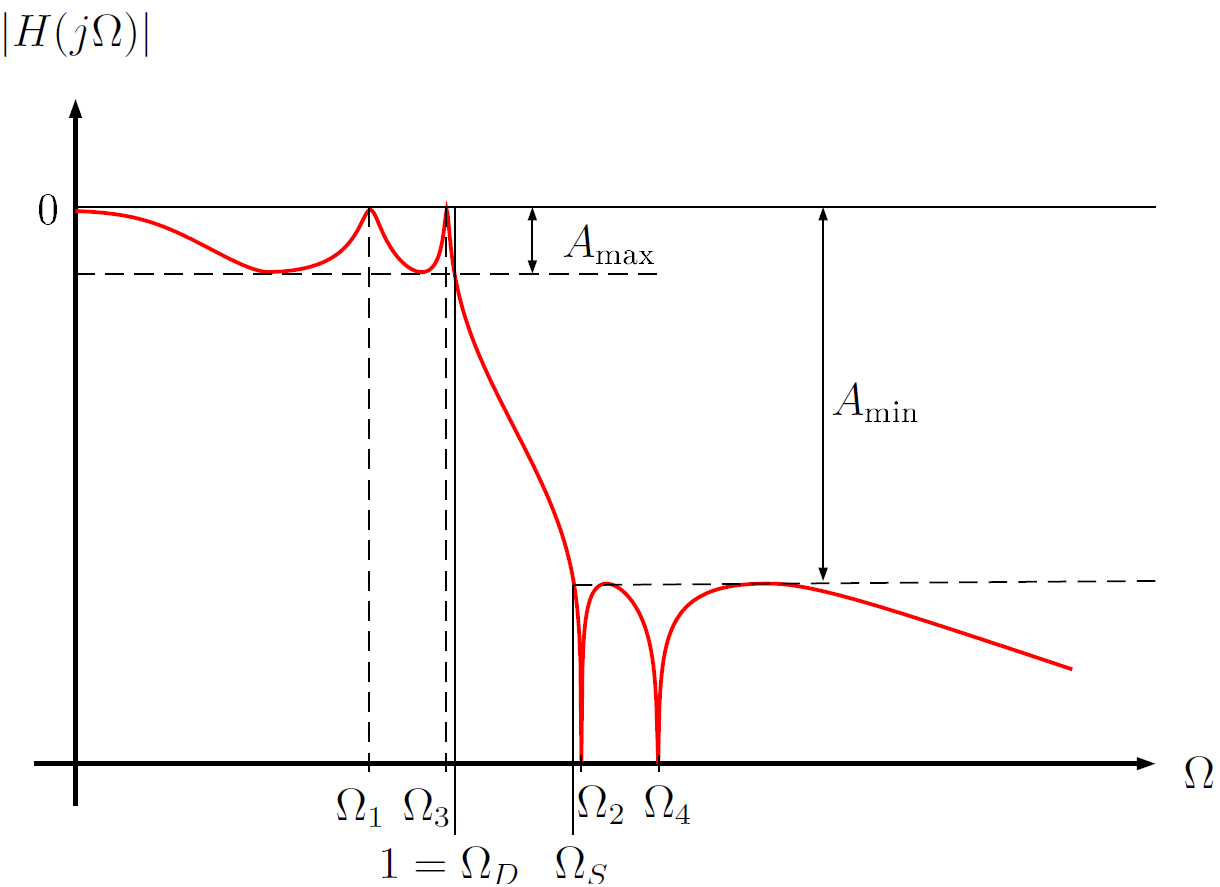
\includegraphics[width=\columnwidth]{images/filter_cauer_amplitudengang.png}
\end{minipage}
\hfill
\begin{minipage}[c]{0.48\columnwidth}
    \textbf{Kombination von Tschebyscheff-\uproman{1} und Tschebyscheff-\uproman{2}}

    Daher spricht man auch von Complete-Chebyshev- oder Chebyshev-Cauer-Filtern (CC-Filter).
\end{minipage}


\subsubsection{Lage der Pole und Nullstellen}{325}

\begin{minipage}[c]{0.4\columnwidth}
    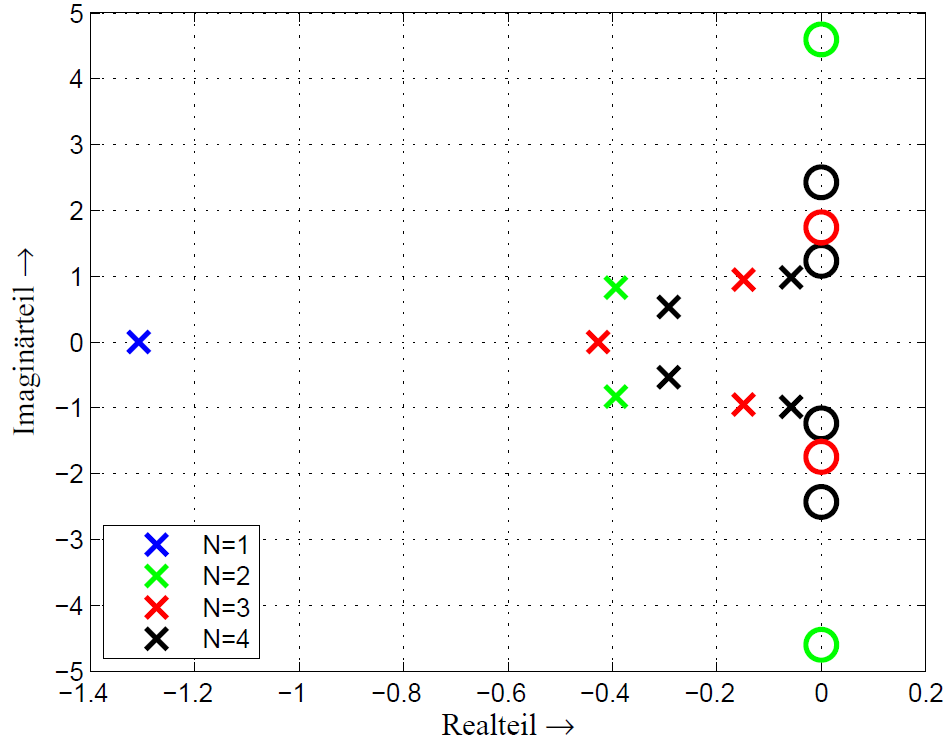
\includegraphics[width=\columnwidth]{images/filter_cauer_pollage.png}
\end{minipage}
\hfill
\begin{minipage}[c]{0.58\columnwidth}
    \begin{outline}
        \1 \textbf{Kein} Allpolfilter
            \2 Gerade Ordnung $n$: $n$ Pole und $n$ Nullstellen
            \2 \textbf{Un}gerade Ordnung $n$: $n$ Pole und $n-1$ Nullstellen
        \1 Nullstellen auf $\jimg \omega$-Achse \textbf{ausserhalb vom Einheitskreis}
    \end{outline}
\end{minipage}


\subsubsection{Filterordnung}{326}

$$ \boxed{ n = \left\lceil \frac{ K \Bigg( \Big( \frac{\Omega_D}{\Omega_S} \Big)^2 \Bigg) \, K \Bigg( 1 - \frac{10^{A_{pass }/ 10} - 1}{10^{A_{stop }/ 10} - 1} \Bigg) }
    { K \Bigg( 1 -\Big( \frac{\Omega_D}{\Omega_S} \Big)^2 \Bigg) \, K \Bigg(\frac{10^{A_{pass}/ 10} - 1}{10^{A_{stop}/ 10} - 1} \Bigg) }  \right\rceil 
    \quad \text{mit } K(k) = \int\limits_{0}^{\frac{\pi}{2} }  \frac{1}{\sqrt{1- k \sin^2(\theta)}} \, \diff \theta }$$
    \textrightarrow\ Nomogramm!


\subsection{Approximation nach Bessel}{328}

\begin{minipage}[c]{0.45\columnwidth}
    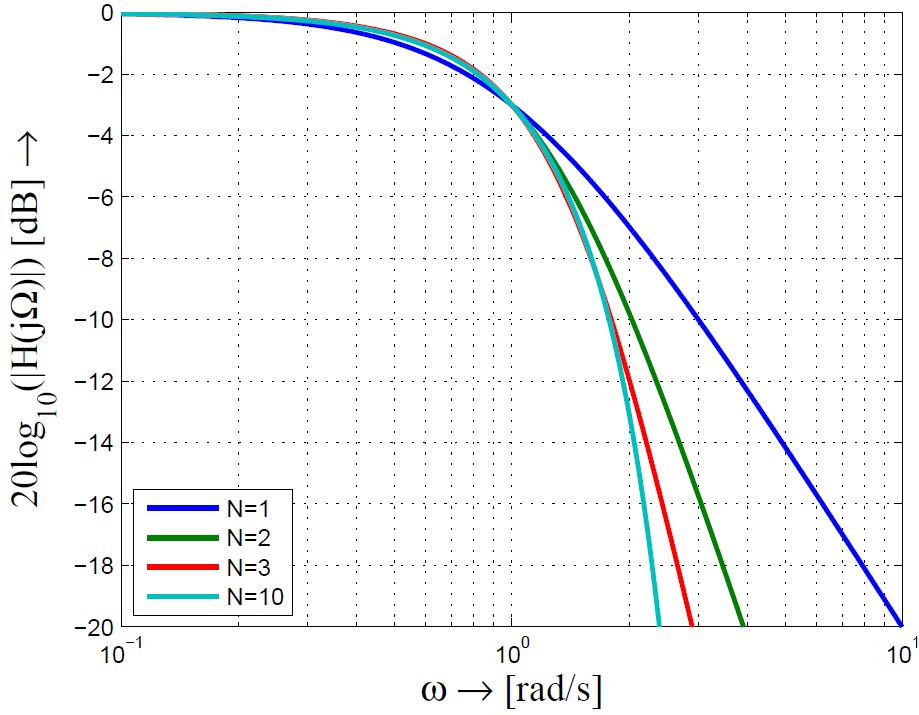
\includegraphics[width=\columnwidth]{images/filter_bessel_amplitudengang.png}
\end{minipage}
\hfill
\begin{minipage}[c]{0.48\columnwidth}
    Bessel-Filter liefern eine möglichst \textbf{lineare Phase}, d.h. eine \textbf{konstante Gruppenlaufzeit}.

    Die Übertragungsfunktion $H(S)$ lautet
    $$ \boxed{ H(S) = K \cdot e^{-S T_0} } $$

    Für die Gruppenlaufzeit folgt somit
    $$ \boxed{ \tau_g(\Omega) = \frac{- \diff \theta(\Omega)}{\diff \Omega} = T_0 = \const } $$
\end{minipage}

\vspace{0.2cm}
Ohne Einschränkung kann in der UTF $T_0 = 1$ und $K = 1$ gesetzt werden:
$$ H(S) = e^{-S} = \frac{1}{e^S} \approx \frac{1}{D(S)} $$


\subsubsection{Gruppenlaufzeit $\tau_g(\Omega)$ und Phasenlaufzeit $\tau_p(\Omega)$}{331}

\begin{minipage}[c]{0.4\columnwidth}
    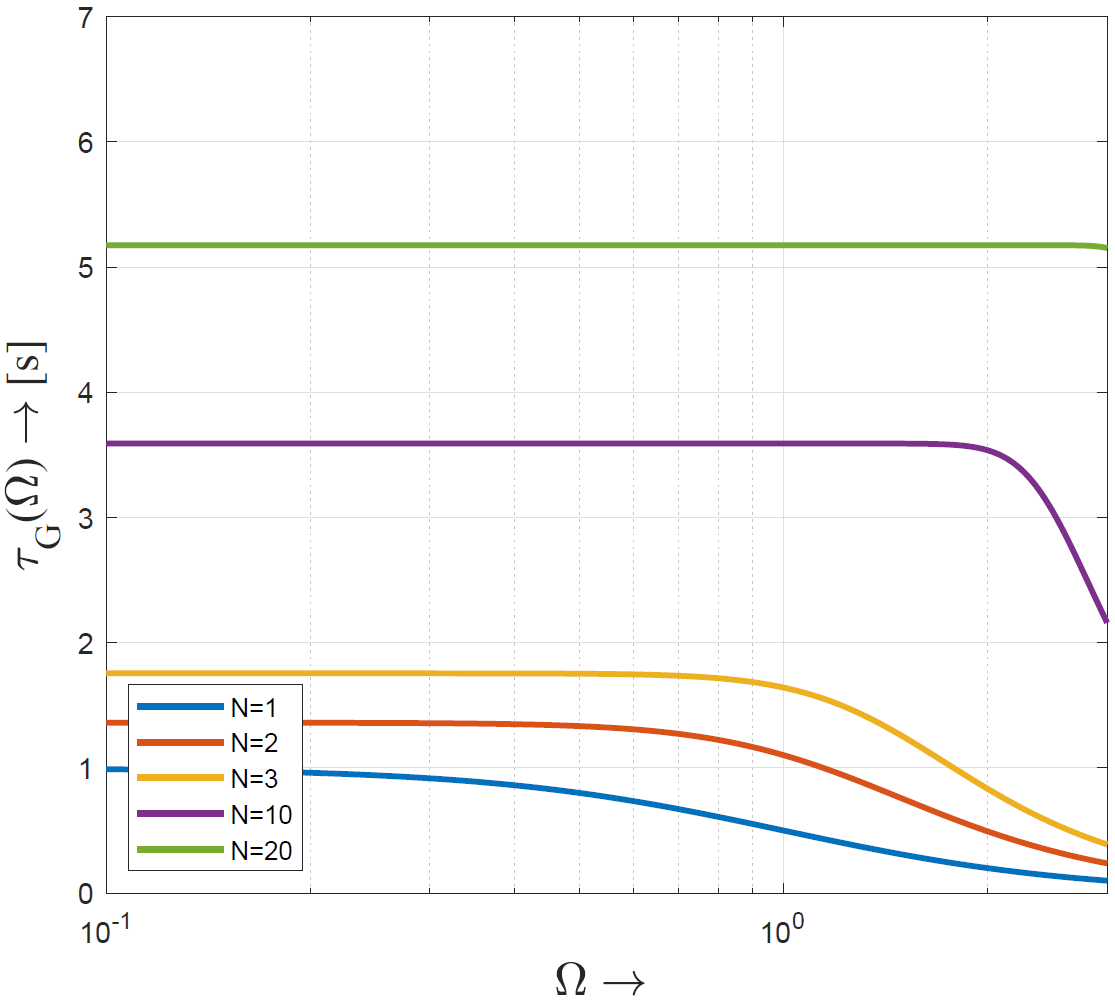
\includegraphics[width=\columnwidth]{images/filter_bessel_gruppenlaufzeit.png}
\end{minipage}
\hfill
\begin{minipage}[c]{0.4\columnwidth}
    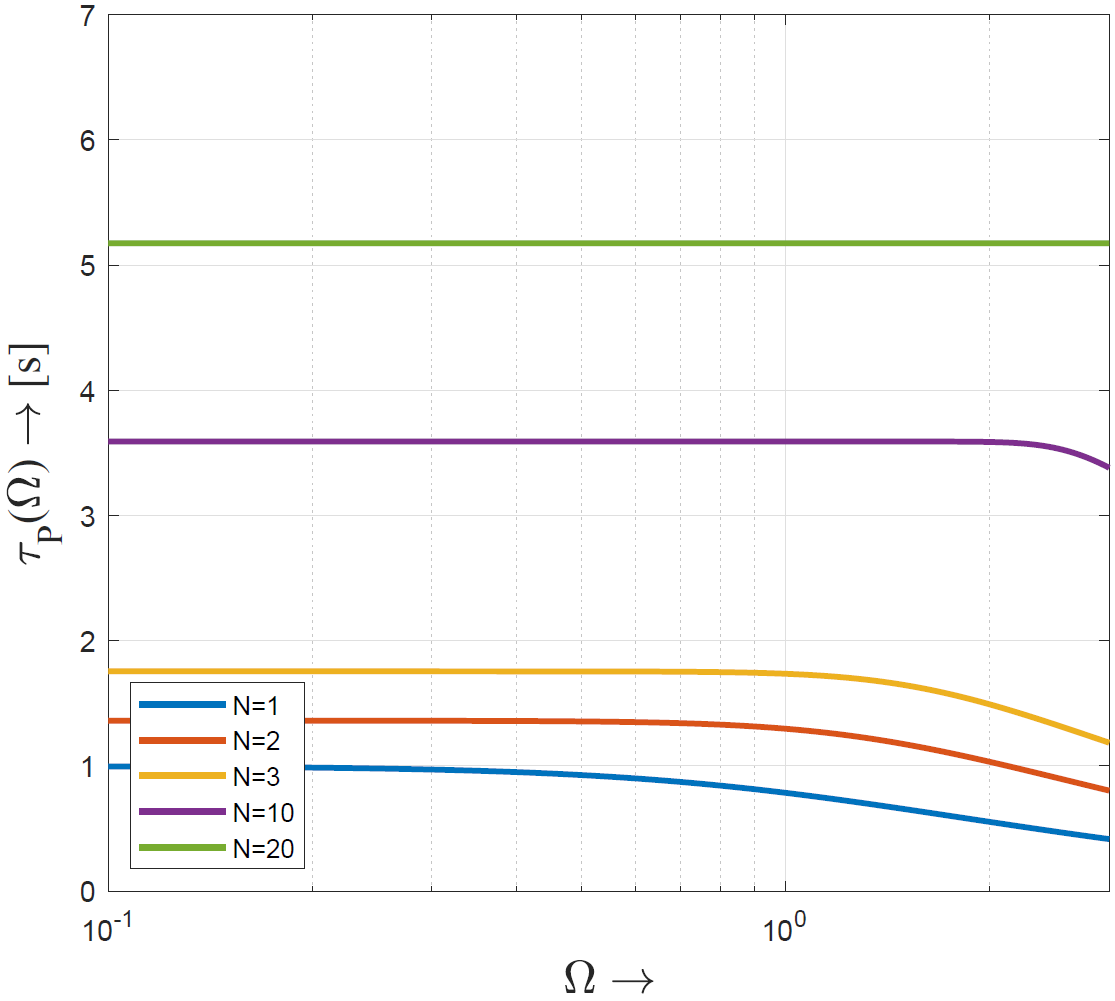
\includegraphics[width=\columnwidth]{images/filter_bessel_phasenlaufzeit.png}
\end{minipage}

